\section{物理基础}
以前数节已讨论过波传播的几何地震学方面的问题,以及它们如何与地震成像有关,现
在我们将考虑其物理方面的问题如何与成像有关.传播介质具有质量密度和可压缩性,讨论
波动要考虑物质的加速度向量和压力梯度.静形变、地滚波、剪切、刚性、能量耗散、成层
沉积——像这样一些因素,与映像的构制有什么关系呢?

因为沉积岩的复杂性,应采用何种数学描述的问题还没有普遍一致的意见。为帮助你认
识起指导作用的理论可以作到什么程度,我将指出理论与现代工业实践之间的一些不一致之
处。

\subsection{碎屑岩沉积剖面}
一般而言,大多数储油岩石都是砂岩-砂岩往往是由水速不足以起搬运作用时在河口附近
沉积的沙所形成。在河口,可发现沙是沿着沙是沿着沙坝的末端沉积下来的,且往往大约为
$25^{\circ}$左右的坡度沉积。如图\ref{fig:xrf/river}所示。尽管沙并非沉积
于平坦地层内,但上述沉积过程却可以形成一种水平地层。
\begin{figure}[H]
\centering
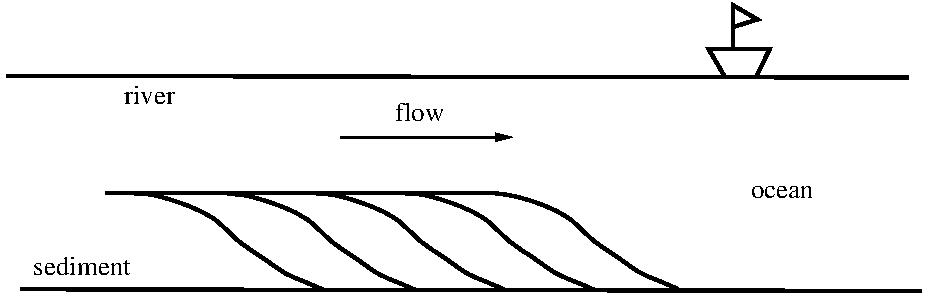
\includegraphics[width=0.5\textwidth]{xrf/river}
\caption[river]{河流入海处相当陡之斜坡上的砂岩沉积(储油岩石)}
\label{fig:xrf/river}
\end{figure}
粘土是甚细粒物质(杂质),在它们沉降而形成页岩之前,被携运至深水区域。页岩沉积
是比砂岩更为水平的一种成层地层。砂岩沉积的具体位置随经过之风暴和季节而变化,在
岩石中留下如木纹年轮状的标记。

由于河道与沙坝经常变化,河流三角洲本身就是一种复杂的沉积,它总是沿着海岸线移
动;在任何一个时期,三角洲似乎都是遗留下沉积物而向海洋方向移动,但是随后发生的沉
降挤压或者海平面升高又可引起它向陆地方向移动。


砂岩很重要,因为它的孔隙能使石油聚集,而它的渗透性能为石油运移形成通道。页岩
也很重要,因为它含有以前时期地球上的生物残迹并因而形成烃类.烃类运移至邻近的砂
岩,但总是不会运移至地面,因为砂岩为无渗透性的页岩所覆盖.尽管页岩具有比砂岩稍微
低一些的速度,可砂岩与页岩的波阻抗性质往往是类似的。地球物理学家要在地面上根据地
震波长的尺度(约30米左右)来观察这最终形成互层的砂页岩三维体。

砂岩页岩混合体称为碎屑岩、碎屑这个词的意是破碎。碎屑岩由结晶岩石的碎片所组
成,多数沉积岩均属碎屑岩,大多数石油是在碎肩岩内发现的,但在与碳酸盐岩有关的岩石
(如灰岩)中也发现了很多石油。碳酸盐岩是在浅海沉积环境由海洋有机物质所形成,许多
碳酸盐岩(及碎屑岩)由于缺乏渗透性而使所含石油难以抽取。经历若干还不太清楚的过程
之后,碳酸盐岩具有了渗透性。地震学家都知道碳酸盐岩具有的速度比碎屑岩速度要大,典型
情形是碳酸盐岩具有比邻近碎屑岩速度太20\%至50\%的速度。碎屑岩有时也包含有灰岩,在
这种情形下,称它为泥灰岩。

\subsection{年代地层学}
看来可能有点奇怪,关于地震反射的准确性质一直没有普遍一致的意见。物理学家倾向
于认为反射是由不同类型岩石的分界面、诸如砂页岩接触面所引起的。这种观在的麻烦
问题是:砂岩与页岩以复杂的方式形成夹层,既可大于也可小于地震波长。许多地质学家,
特别是以地震地层学家而知名的一群地质学家,他们有一种不同的概念(见美国石油地质学
家协会第26号研究报告:地震地层学一在油气勘探中的应用),他们曾经研究过成千英里
的具有测井资料的反射资料,相信一个反射是标志着一个恒定地质年代的地层。他们证实一
个连续追踪很长的反射面可以在一段是代表陆源沉积而另一端则是代表海相沉积,二者之
间可以有各式各样的岩石类型建立。在这种假说基础上的资料解释方法就称作年代地层学。
在整个全是碎肩岩沉积的地区震池层学家的观点看来是相当正确的。但是当存在有碳酸
盐岩和其它岩石时,物理学家的点看来要更为适宜,要进一步详细研究,建议读者读一读
Sheriff (1980)所著的书。

\subsection{转换横波难以观测}
在夭然地震学和实验室观测中,可清楚地观察到存在两种波速,速度较快者为压力波
(P波)而速度较慢者为横波(S波)。横波可随水平平面内的地面运动而呈极化(SH
波),或者在垂直平面内极化波)。理论、野外资料及实验室测定等结果均符合一
致。Cherify与Waters(1968)以及Erickson, Miller与Waters等人(1968
)曾经成功地在勘探环境条件下采用S波进行了试验工作。

值得注意的是,99\%以上的石油勘探工作均忽略了横波之存在。在数学上,是把地层当
作是一种流体或一种气体来进行处理的。横波试验工作采用专用设备来产生和记录垂直于测
线方向的振动、即SH波。由这些横波得出的地层图像往往为土壤层所削弱,但有时SH波
图像却清晰而一致。奇怪的是,纵使是良好的SH波资料也总是难于与P波图像对比。这些
试验研究表明,除了在土壤层中之外,典型情形下的横波传播速度大约为压力波的二分之
一,而在土壤层中,横波速度总是慢得多而且变动更大。观测到的横波通常具有比压力波低
的频率,其频率与速度均为压力波之二分之一的一种横波应正好具有与压力波相同的波长,
从而也就应具有与压力波相同的分辨能力。试验工作确实证明,横波可提供大约与压力波相
同的空间分辨能力,大多数地面地震资料只表示运动的垂直分量,而所有海上地震资料则是
记录压力波,所以,在常规的观测排列情形下,我们理应从来观察不到波,更精确地
说,SH波应很微弱,仅仅是由地层偏离简单的成层情形所形成。

反射地震学中有关横波的令人费解之问题是:石油勘探人员采用标准的野外观测系统按
常规方法观测由$P$波至$S$波的转换,这种企图失败了;而理论却预言以某种角度入射
在分界面上的$P$波应局部转换成$SV$波。再者,在通常所遇到的以$30^{\circ}$至
$60^{\circ}$角度入射的反射波这种情形下,这些转换波具有可与$P$波相比拟的强弱
范围。

常规的观测排列和处理在某种程度上是要削弱转换横波的,但是它也削弱多次反射(处
理方式非常相同),而我们是随时都可遇到多次波的。再者,转换波的波形特征类似于多次
波,可是二者是显著不同的两种波。转换波通常在速度测定中应有所显示(见第三章),图
\ref{fig:xrf/africa}所示是一种含有某些多次反射的零炮检距剖面,多次反射很容易
识别出来,因为它同较浅深度的地形模样完全相同。转换波将重复这种地形模样但时间标度
比例将穴约是3/2而不会严格等于4/2。在具有一种像图\ref{fig:xrf/africa}所示的
充分复杂的地形条件下,把转换波误认为是另一种一次反射的可能性将是很低的。
\begin{figure}[H]
\centering
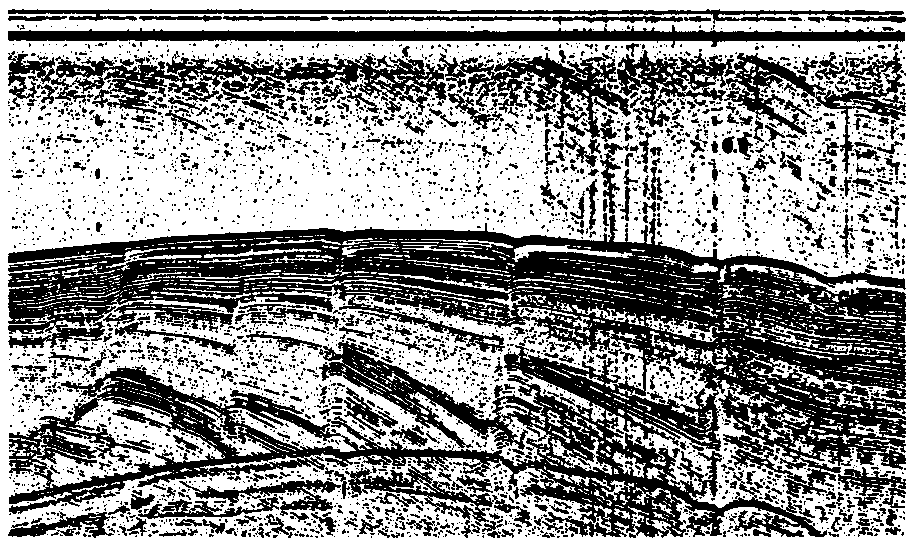
\includegraphics[width=0.5\textwidth]{xrf/africa}
\caption[africa]{东非地区带有多次反射的零炮检距剖面}
\label{fig:xrf/africa}
\end{figure}
在勘探中,转换波理应具有良好的判断价值,不过,在常规资料中观察出转换波的可能
性看来还相当渺茫,以致大多数解释人员都放弃了这种打箅。为什么在常规资料中观察不出
转换波?可以列举出若干理由:
\begin{enumerate}
\item
  在海上地震勘探资料中,因传播路径经过海水层,必然再度转换为$P$波;
\item
  在陆地资料中,表层土壤特别易于吸收横波能量;
\item 垂直分量检波器利于观测$P$波不利于观测$S$波,在近地表处因射线趋宁垂直,尤其
是如此。
\end{enumerate}

上述转换波为何会弱于压力波的所有理由中,没有一个是占有优势地位的。在广泛变化
的环境内记录到范围广泛的振幅,记录数据总是采用自动增益控制(AGC)加以显示,弱
振幅似乎尚不足以引致观测失败。关于这个问题,我们应继续注意研究,转换波应用于解释
无疑会比我们所承认的更为盛行(我还从未在常规记录上识别出转换横波)。

所以,虽然转换横波某天在反射地震学中起一种重要作用,可我们现在最好还
是转向讨论主流问题吧——如何有效处理常规观测的资料。

\subsection{混响模拟的可靠性}
地震学文献包括有大量关于成层介质内的地震波理论的讨论,应用地震学的一个值得注
意的问题是:一般均将层间内部的混响忽略不计。当波从一个分界面反射时,反射波强度只
等于入射波强度很小的一部分,典型的是小于10\%,这种反射波就是本书主要讨论的一种
波,然而,反射波本身还会反射而又反射,直至反射无限多次。对于短路程情形,可以有非
常多这样的射线。问题是这些混响是否总能累积达到足以值得去考虑它们的程度。看来答案
就是:这类混响虽可能有意义,可是地震学家很少能够用这种具体体现混响的相当复杂的理
论来改善反射地震勘探资料的解释工作。若干更详尽一些的讨论,可阅读5.5节。

当有测井记录可资利用,情况会有些改进,不过,这时也还存在有严重的困难。
处理之后最可能获得的横向分辨率大约为20米至50米,然而,测井记录并不是一种具有20米
呈50米数量级横向分辨水平的地层。你若观察过一个由高速公路切割出来的沉积剖面就会懂
得,一个点和一种横跨20至50米范围的横向水平之间是有很大差别的。在实际应用中,人们
都要对测井记录进行垂向平滑处理,过小的平滑会得出过多的混响,过多的平滑又会得不出
混响。垂向平滑的数量级是一个靠经验决定的参量,它对所得结果有显著影响。对测井记录
进行垂向平均不一定能满意地趋近所平分辨率。

\subsection{牛顿粘滞性理论的失败}
同样值得注意的问题是:地震学基本教科书在解释能量耗散参量Q值的频率依从关系时
遇到失败。关于能量耗散问题,最简单的理论处理办法必须对阐述应力与应变关系的胡克定
律加上一顼应变率。这种理论预言:高频能量相对耗散应比低频能量相对耗散强一些。可是
实验上观测到的却是:在几十赫兹频率范围上,相对能量耗散大略是恒定的。另一些简单的
牛顿理论则以$-i\omega$的多项式比值来描述应力与应变之比,这些理论均包含宥比例
长度及特征频率。它们都未预言Q值为常数。看来,一切比例尺度的岩石不均勻性似乎应该
成为一种成功的理论所应包括的本质属性(4.6节讨论的即属此种情形)。

\subsection{反演问题基本特点}

物理过程经常可用计算机按其自然面目进行模拟,计算机内存犹如是物理空间的图形,
而计算中的时间发展演化则犹如是所模拟的现实世界中的时间过程。按这种方式求解问题有
一个好处,就是没有任何关于解的唯一性的疑问,原始数据与模型离散化的误差不太可能造
成灾难性的影响。可是,勘探地球物理学家极少求解这类问题。我们通常不是把$(x,z)$空
间放在计算机内存中并令时间$t$演化发展,而是把$(x,t)$空间放在内存中并沿深度$z$方向进
行外推,根据地面上的信息(数据资料)试图外推出一定深度上的信息,这才是我们的正
事,稳定的财间演化发展过程实质上并未提供能够保证我们的外推目标是合理的、稳定的
或甚至是可能的“存在性证明”。

时间演化发展问题经常称作正演问题,而深度外推问题则称作反演问题,在正演问题
中,诸如在利用纵波进行的一种正演问题中,你需要什么和你能得到什么,都是很清楚的。
你需要岩石的密度$\rho(x,z)$和不可压缩性模量$K(x,z)$,而且你需要知道初始的震源分
布。你能得到晚些时刻时各处的波场,不过你通常只是要地表面上的波场,以便于同某些资
料进行比较,在反演问题中,你已知的是震源特性和地面上所观察到的波,你想要确定表
征物质性质的$\rho(x,z)$和$K(x,z)$。根据经验已经知道,常规的观测结果是得不出有关
$\rho$与$K$之映像或图形的合理估计的。

\subsection{你能从反射地震学得到什么}
很幸运,已经发现$\rho$与$K$的某种函数能够可靠地加以确定并绘制成图。速度$v$与波阻抗
$R$由下式给出
\begin{subequations}\label{eq:ex1.4.1}
\begin{equation}
v=\sqrt{K/\rho} \label{eq:ex1.4.1a}
\end{equation}
\begin{equation}
R=\sqrt{K\rho} \label{eq:ex1.4.1b}
\end{equation}
\end{subequations}
从数学上说,要反向求解式\ref{eq:ex1.4.1}是件容易的事,由此得
\begin{subequations}\label{eq:ex1.4.2}
\begin{equation}
K=vR \label{eq:ex1.4.2a}
\end{equation}
\begin{equation}
\rho=R/v \label{eq:ex1.4.2b}
\end{equation}
\end{subequations}
实际应用时,式\ref{eq:ex1.4.2}这种解没多大价值,因为$v$与$R$这两个参量是通过无重迭部分的频
谱范围来观察的。波阻抗$R$通过质量良好的反射资料典型频宽为$10Hz$至$100Hz$的频谱范围来观察到,
观测到,由于丢失了谱的低频部分,平常都不是说观测波阻抗而是观测其梯度,即反射率$c(x,z)=\nabla log(R)$。

速度$v$是通过非常窄的频宽范围观测到的。速度观测涉及要对旅行时间随炮检距而变化
的情形进行研究,这将在第三章内详加讨论。利用这个第二种频宽范围是难以在一个4秒长
的时间轴上辨认出十六个独立的速度测定的,所以这种频宽范围就是从零至大约2赫兹\footnote{4秒长的时
间上可辨认出16个速度测定结果,其平均时间间隔$\Delta t=250$毫秒,根据读数定理,其频率最高为
$1/2\Delta t=\frac{1}{2\times 0.25}=2$赫兹。——译者},如图\ref{fig:xrf/rely}所示。
\begin{figure}[H]
\centering
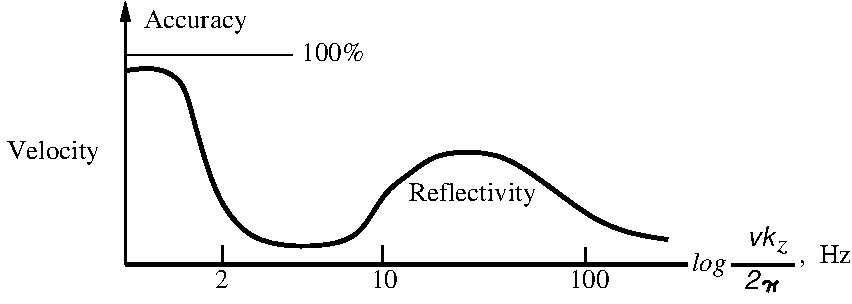
\includegraphics[width=0.5\textwidth]{xrf/rely}
\caption[rely]{根据地面地震观测所得信息之可靠性程度}
\label{fig:xrf/rely}
\end{figure}
注意,从2赫兹至10赫兹,存在有一个信息空白段。即使假设岩石物理学可以给我们提供密度$\rho$与
不可压缩性系数$K$之间的关系,这个空白也会严重妨碍地震学家在进行钻井之前就能预测测井记录情况
的能力,地震学家能够作得可靠一点的只是对已经过滤波处理的测井记录进行预测而已。

上述观测情况使得反射地震学家不得不把“速度”这个词当作一个专用术语来用了。对
反射地震学家来说,速度的意思就是指“真速度”的低空间频率部分,“真速度”的高频部分
从未称作速度,而是称作反射率(reflectivity)。密度由于几乎无法根据地面反射地震学
来测定,通常都不注意它。

\subsection{数学反演问题}
在数学中,求解一个反演问题的意思就是根据波场来“决定”介质性质,往往是采用一
个“收敛序列”来达到这个目的。而地球物理学所指的“决定”究竟是什么意思却不太严谨
(或者包括内容太多)。在本书的第一章至第二章中,反射面是根据自激自收概念“决定”
的;在第三章中,又同炮检距结合起来了,反射率与速度则以观测排列延拓的概念
来“决定”;在第五章中,这种概念发展为抑制多次反射然后再令下行波初动时间以前出现
的上行波等于零的办法来求取反射的“真”振幅。看来很可能未来的处理方法还要形成一些
其他成像概念,也许有可能证明我们的某些“决定”同数学家的那些“决定”是符合一致
的,但是这样的符合一致并不是我们的目标。

\subsection{声波波动方程的导出}
声波波动方程描述液体内或气体内的声波,另一种更复杂的方程组描述固体中的弹性
波。现在从声波情形开始讨论。牛顿动量守恒定律说,气体之内的一个小体积将因有力的作
用而加速,力由小体积的相向两端上的压力差所形成。现定义\\
$\rho$=流体每单位体积的质量;\\
$u=x$方向的流体流动速度;\\
$\omega=z$方向的流体流动速度;\\
$P=$流体内之压力;\\
牛顿定律说:\\
质量$\times$加速度=力=$-$压力梯度\\
\begin{subequations}\label{eq:ex1.4.3}
\begin{equation}
\rho\frac{\partial u}{\partial t}=-\frac{\partial P}{\partial x} \label{eq:ex1.4.3a}
\end{equation}
\begin{equation}
\rho\frac{\partial\omega}{\partial t}=-\frac{\partial P}{\partial z} \label{eq:ex1.4.3b}
\end{equation}
\end{subequations}
因压缩与体积变化而形成能量储集是第二种物理过程。如在$x+\Delta x$点上的速度向量
$u$超过在$x$点上的速度,则说流动是发散的。换言之,$x$与$x+\Delta x$之间的小
体积正在膨胀。这种膨胀必然导致有一压力降,压力降的大小与称作不可压缩性系数尺的
流体性质成比例,在一维情形下,该方程为\\
压力降=不可压缩性系数$\times$速度之散度\\
\begin{subequations}\label{eq:ex1.4.4}
\begin{equation}
-\frac{\partial P}{\partial t}=K\frac{\partial u}{\partial x} \label{eq:ex1.4.4a}
\end{equation}
在二维情形下则为
\begin{equation}
-\frac{\partial P}{\partial t}=K(\frac{\partial u}{\partial x}+\frac{\partial \omega}{\partial z}) \label{eq:ex1.4.4b}
\end{equation}
\end{subequations}
为从式\ref{eq:ex1.4.3a}与\ref{eq:ex1.4.4a}得出一维波动方程,首先用$\rho$除式\ref{eq:ex1.4.3a}并对$x$求导
\begin{equation}
\frac{\partial }{\partial x}\frac{\partial}{\partial t}u=-\frac{\partial}{\partial x}
\frac{1}{\rho}\frac{\partial P}{\partial x}
\label{eq:ex1.4.5}
\end{equation}
其次,对式\ref{eq:ex1.4.4}取时间导数。在固体地球科学中,我们很幸运的是问题中的
物质在我们进行试验期间并不改变,这意味着$K$不是时间$t$的函数
\begin{equation}
\frac{\partial^2 P}{\partial t^2}=-K\frac{\partial }{\partial x}\frac{\partial}{\partial t}u
\label{eq:ex1.4.6}
\end{equation}
将式\ref{eq:ex1.4.5}代入式\ref{eq:ex1.4.6},得一维标量波动方程
\begin{subequations}\label{eq:ex1.4.7}
\begin{equation}
\frac{\partial^2 P}{\partial t^2}=-K\frac{\partial }{\partial x}
\frac{1}{\rho}\frac{\partial P}{\partial x} \label{eq:ex1.4.7a}
\end{equation}
在二维空间内,准确的声学标量波动方程为
\begin{equation}
\frac{\partial^2 P}{\partial t^2}=K(\frac{\partial }{\partial x}
\frac{1}{\rho}\frac{\partial P}{\partial x}+\frac{\partial }{\partial z}
\frac{1}{\rho}\frac{\partial P}{\partial z} )\label{eq:ex1.4.7b}
\end{equation}
\end{subequations}
你经常会见到简化形式的标量波动方程,在这种形式的方程中,假设$\rho$不是$x$与$z$的函数,采
用这种近似一般有两个理由:一是因观测结果一般都不能确定密度,所以最好是把密度取为
常数;二是如果该系数是空间变量的函数,傅氏变换方法求解就无法适用了。在考察这种近
似是否成立之前,先考察一下由此会得何种结果。采取这种近似,直接就可将式\ref{eq:ex1.4.7b}
简化成标量波动方程的通常形式
\begin{equation}
\frac{\partial^2 P}{\partial t^2}=\frac{K}{\rho}(\frac{\partial^2}{\partial x^2}+
\frac{\partial^2}{\partial z^2})P
\label{eq:ex1.4.8}
\end{equation}
代入试验解
\begin{equation}
P=\exp (-i\omega t+ik_xx+ik_zz)
\label{eq:ex1.4.9}
\end{equation}
就可看出这个方程不过是重述前数节中的儿何概念,所得就是二维波动方程的波散关系
\begin{equation}
\frac{\omega^2}{K/\rho}=k_x^2+k_z^2
\label{eq:ex1.4.10}
\end{equation}
早先(1.2节式\ref{eq:ex1.2.8}),只考虑波的几何性态就建立过类似于式\ref{eq:ex1.4.10}的方程。在那
种处理办法中,已经发现式\ref{eq:ex1.4.10}
中的$K/\rho$就是波速的平方根。物理学与几何学就这样
经由下列联系而和谐一致了
\begin{equation}
v^2=\frac{K}{\rho}
\label{eq:ex1.4.11}
\end{equation}
最后,让我们看一下为什么在速度是空间可变时就不能采用傅氏变换方法。设$\omega$、$k_x$与$k_z$均是
非空间坐标的函数,将\ref{eq:ex1.4.9}式代入\ref{eq:ex1.4.8}式内,于是你就得到矛盾结果;如
果速度是空间坐标的函数,那么$\omega$、$k_x$与$k_z$就都必须是空间可变的。再假设它们全具有空间
可变性,于是所得方程将仍然是一种偏微分方程,而不是像式\ref{eq:ex1.4.10}那样的一种代数方程。

\subsection{倏逝波与地滚波}
完成波散关系的物理推导,得
\begin{equation}
k_x^2+k_z^2=\frac{\omega^2}{v^2}
\label{eq:ex1.4.12}
\end{equation}
我们现在可以对它有一种新考虑,它带来了远比早先根据几何推导所能设想到的更为多的意
义。原先只不过把波散关系看成是体现一种几何关系$cos^2\theta+sin^2\theta=1$,其中
所以$sin\theta$超过1是没有意义的,换言之,$vk_x$超过$\omega$是没有意义的。现在在这里却是有意义
的,前面述及两种偏移方法中都隐藏了一个未加解释说明之赴,既然数据资料可以是$(t,x)$
平面中的一个任意函数,那么它的傅氏变换当然就可以是$(\omega,k_x)$平面内的一个任意
函数了,于是,实际上总是存在有角度的正弦会大于1的能量,这种情形如图\ref{fig:omk/evtheory}所示。应
该怎么对待这种能量呢?
\begin{figure}[H]
\centering
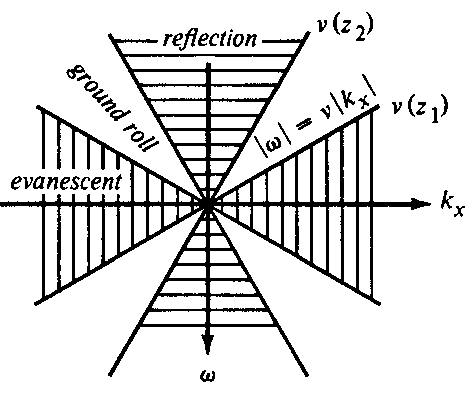
\includegraphics[width=0.5\textwidth]{omk/evtheory}
\caption[evtheory]{反射能量的三角形区域$|\omega|>v(z)|k_x|$随速度$v$的增大,因而
也就是随深度$z$的增大而变得更窄。地滚波是沿地面传播的能量,而指数衰减波则是地下深处传播的
能量}
\label{fig:omk/evtheory}
\end{figure}

$vk_x$在超过$\omega$时,最好将熟悉的向下外推算子改写成
\begin{equation}
e^{\pm i\sqrt{\omega^2/v^2-k_x^2}}\cdot x=e^{\pm\sqrt{k_x^2-\omega^2/v^2}}\cdot x
\label{eq:ex1.4.13}
\end{equation}

这个式子说明,物理解的深度依从关系是一种增长指数形式或一种阻尼指数形式,这些解称
作倏逝波\footnote{原文为evanescence,直译应为“消散波”或“耗散波”,“倏逝波”这种波具有按指数规律迅速变化的性质,而且有意义的是按负指数规律变化的波。——译者}(evanescent wave)。在最极端情形$\omega=0$时,$k_x$是实数,从而$k_x=\pm ik_x$。
对于弹性波,这点可用地面在一架停泊飞机的作用下所发生的形变来举例说明。仅当飞机运动速度高
于波在地层内之传播速度时,才会有一个波辐射进入地下。如飞机以亚音速运动,这时发生
的形变叫作准静态形变。

以具有正弦形皱纹的薄板进行假想试验,也许是一
种比较好的物理描述方法。这样的金属薄板有时用作房
顶或汽车库大门。皱纹之波长固定了$k_x$值。这样的薄板
以速度$V$运动经过你耳朵时,不论$V$是否大于还是小于
空气中的声速,你都会听到一种振荡频率等于$Vk_x$的声
音,但是你听到的声音将随离开该薄板之距离而指数衰
减,除非它运动得非常之快$(V>v)$。在这种情形下,
运动着的薄板辐射出的声音会达到很远距离。这就是超
音速飞机为什么使用如此大量燃料的原因。

偏移程序对运动速度低于声速的能量应该有什么影
响呢?理论上,这种能量应当沿着离开震源远去的方向
作指数衰减,在$(\omega,k_x)$空间抑制带区域内的阻尼衰
减极快速。因而,简单的爆炸反射面理论预言,在速度
低时,资料内应该几乎就不存在能量。

但是真实情形是:$(\omega,k_x)$空间的指数衰减区域内不是有极少量能量,而总是存在大
量能量,爆炸反射面概念又一次破产了。处理陆地地震资料时,问题更糟糕。在深处速度
较快的岩石内作指数衰减的波可以在低速土壤层中传播,这种能量称作迆滚波,图\ref{fig:omk/evdata}
是一个例子。像起伏变化很大的地表面一样,控制着地滚波的最浅地下界面也是变动很大
的,所以虽然图\ref{fig:omk/evdata}是一个好例子,但没有一个例子可以真正是典型的。
这个资料不是零炮检距剖面,炮点在左侧,而右侧各记录道则由离炮点距离逐渐増大的裣波器所产生。图上
绘有直线,其斜率相应于海水层的速度,较陡的同相轴全是地滚波。在这张图中,存在两类
地滚波。有一类其速度大约等于海水层速度的一半;振幅较强的一类其速度大约等于海水层
速度的四分之一,该种到达较迟而振幅较强的一类地滚波具有以频散现象而知名的有趣恃
征,从上下关系来观察该资料,你应能注意到高频到达早于低频。
\begin{figure}[H]
\centering
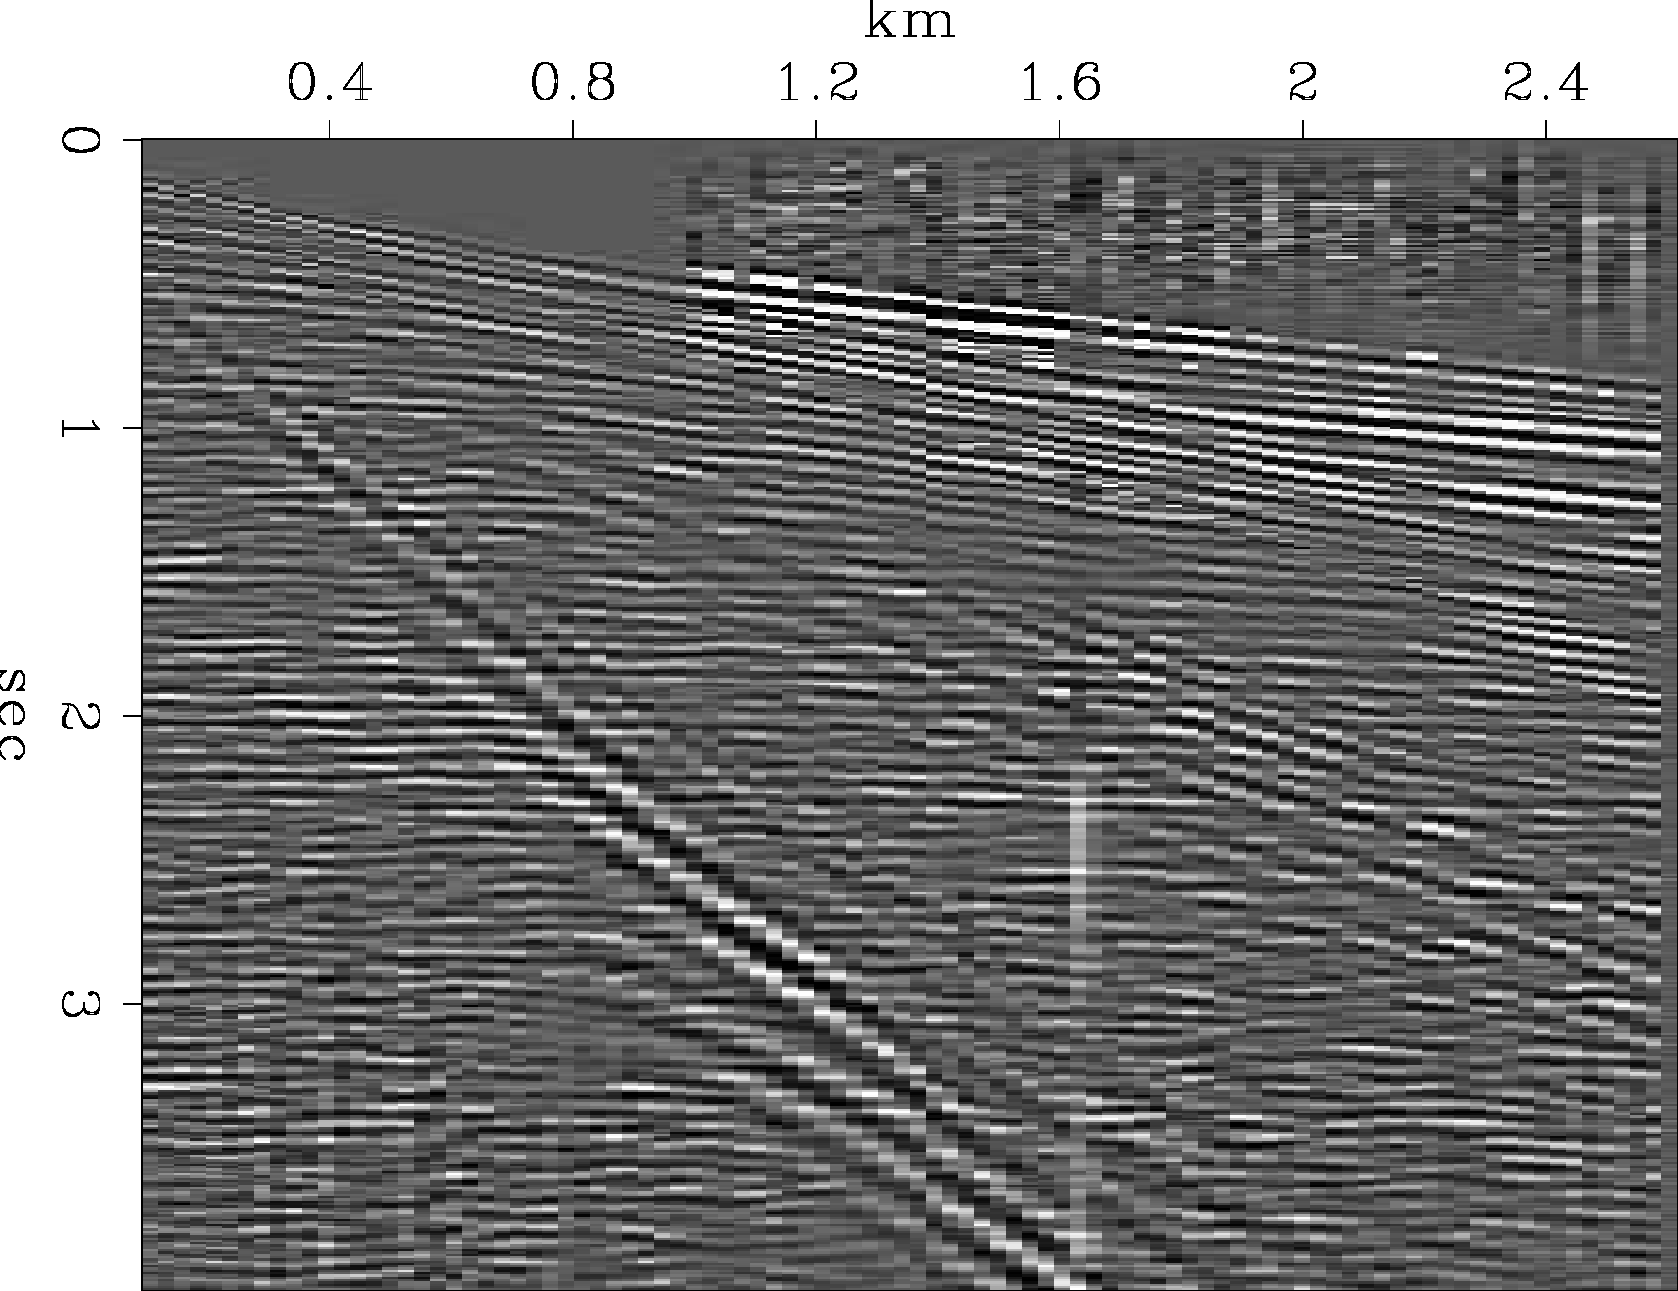
\includegraphics[width=0.5\textwidth]{omk/evdata}
\caption[evdata]{佛罗里达浅海地震剖面,显示具有频散现象的地滚波}
\label{fig:omk/evdata}
\end{figure}
由于地滚波指数衰减有效地防止了它受深层目的层的影响,所以地滚波成了不受欢迎的
干扰。在实际处理中,应使$(\omega,k_x)$空间抑制带区域内的能量衰减掉,用数学语言描述就是
说,从模型空间至数据空间、然后又返回模型空间的这种合成映像过程,不是一种恒等变换
而是一种等幂变换。
\subsection{反射与高频极限}
众所周知,两种不同物质的接触面可以引起反射。不可压缩性系数AT或密度P以空间阶
跃函数形式改变的地方,就定义为物质接触面。在一维情形下,$\frac{\partial K}{\partial x}$、$\frac{\partial\rho}{\partial x}$或者二者会在某
一点上成为无限大,并且我们知道,任一种都可以形成反射。所以,也许有点奇怪,密度的
导数是明显出现在式\ref{eq:ex1.4.7b}内,而不可压缩性系数的导数却未明显在该式中出现,
这意昧着略去式\ref{eq:ex1.4.7b}中的密度梯度,并不会消去所有可能的反射。可是,略去该项会使进
一步的分析稍微简化,而且因为恒定密度是一种合理的情形,所以总是略掉该项的。

还存在有一些众所周知的数学条件,在该条件下,一阶项均可略去。现在集中注意一个
沿任何特定方向传播的波,这时,$\omega$,$k_x$和$k_z$都有某种规定的值。
在频率趋向无限大的极限情形时,式\ref{eq:ex1.4.8}内的诸二阶导数项$P_{11}$、$P_{xx}$与$P_{xx}$
均趋于无限大的二次幂。假设两种介质逐渐彼此混合,从而使密度梯度小于无限大,于是式\ref{eq:ex1.4.7b}导出式\ref{eq:ex1.4.8}时出现的形式为$\rho_xP_x$与$\rho_xP_x$的一阶导数乘积项,均可忽略不计,因为这些项在频率趋向无限大时仅趋于无限大的一次幂,因而可在该种极限情形下将其忽略不计。

目的在于计算合成地震记录的理论地震学中,通常要包括这些项,但在目的在于根据地
震野外数据作出地层模型的场合——如本书中的场合——一般是忽略这些项的。地层成像
比计算合成地震记录要困难得多,忽略这些项的理由往往只不过是为了减少麻烦;为将方程写
成二维而不是三维形式(推广至三维通常是可能的,但往往并不要求如此),根据同样的理
由也能忽略这些项。此外,总是要忽略这些项以便于采用傅氏变换方法。也许会出现需要这
些项使之包括在内的实际情况,如果是这样,采用有限差分方法(见2.2节)不难将它们包
括在内。但是任何企图将它们包括在数据处理之中的努力,也应当注意考虑具有类似意义的
其它因素,诸如要假设声波方程可以近似应用于弹性介质情形等等。

\subsection{习题}
\begin{enumerate}
\item 在一定深度的潜水面之下,土壤为水所饱和是典型情形。采用重锤地震仪记录系
统的工作经验证明,地震波速度的典型情形是在潜水面上突然跃变为水的速度($V_{water}=
m/s$)。据说,在一定位置上观察到地滚波要比反射波强一些,所以决定把检波器埋置在地
面下。观测到这种引起麻烦的地滚波的传播速度等于水的速度的十分之六。要使地滚波衰减
十倍,试问检波器必须埋置潜水面之下多深?假设所帶数据资料已包含从10赫兹至100赫兹
的所有频率。(提本:$log_e^{10}\approx 2$,$2\pi\approx 6$等等)
\item 设有一维波动方程
\begin{equation}
(\frac{\partial^2}{\partial t^2}-\frac{K(z)}{\rho(z)}\frac{\partial^2}{\partial z^2})P=
-\frac{K(z)}{\rho(z)^2}\frac{\partial \rho}{\partial z}
\frac{\partial P}{\partial z}
\label{eq:ex1.4E1}
\end{equation}
现考虑以下列函数作为试验解
\begin{equation}
P(z,t)=P_0\frac{1}{\sqrt{Y(z)}}\exp(i\omega t-i\int_0^x\omega\sqrt{\frac{\rho(\xi))}{K(\xi)}}d\xi)
\label{eq:ex1.4E2}
\end{equation}
式中\\
$P_0=const.$\\
$Y\equiv\frac{1}{\sqrt{\rho(z)K(z)}}$\\
将试验解\ref{eq:ex1.4E2}代入波动方程\ref{eq:ex1.4E1},试讨论在物性参量允许变化与不同波长情形下的解
均能成立这两种要求之间应如何权衡折衷。
\end{enumerate}



